% !TeX encoding = UTF-8

\chapter{REVISÃO BIBLIOGRÁFICA}\label{ch:rev-bibs}

Vários trabalhos serviram como fonte de conhecimento e suporte para o entendimento e desenvolvimento deste tema. Alguns foram considerados mais importantes por abordar detalhadamente o problema de reconhecimento, outros foram buscados para se entender melhor, ou ter outra visão sobre alguns detalhes específicos do problema.

Trabalhos de autores como \cite{geysilva} ajudaram a estruturar e organizar o tema por abordar tópicos similares e por possuir riqueza de detalhes no assunto de análise de componentes apresentando uma implementação em \textit{MatLab} (um \textit{software} interativo voltado para o cálculo numérico).

O trabalho de \cite{img-digital-willians} foi utilizado para se aprofundar no tema de imagens digitais, assim como  \cite{gonzalez_woods} que também esclareceu o funcionamento de escalonamento, normalização e mono cromatização de imagens. O autor Dr. Andrew Davison em seu livro \cite{drmathew_java_programming} se destacou pela ótima didática facilitando o entendimento de Análise de Componentes e sua relação com \textit{EigenFaces}. 

Os trabalhos \cite{tutorial_en_smith} e \cite{tutorial_pt} foram estudados como tutoriais do processo de ACP e serão usados posteriormente como guias de implementação do algoritmo.

Nas próximas seções serão explanados os conteúdos destes e de outros trabalhos.


\section{Conceitos de Aquisição e Processamento de Imagens}\label{sec:processamento_imagens}

Com a abrangência dos sistemas de comunicação, com difusão de conhecimentos informações pelos diversos meios, captar, armazenar e processar imagens se tornou necessidade fundamental. Para o reconhecimento de faces em vídeo, o sucesso deste processo é pré-requisito  para o funcionamento dos algoritmos. 

As sessões a seguir contemplam fundamentos básicos sobre imagem, vídeo, a alguns de seus processamentos necessários para a aplicação dos algoritmos de detecção e reconhecimento de faces.


\subsection{Imagem Digital}\label{subsec:imagem}

A imagem digital são valores numéricos disponibilizados em uma matriz bidimensional. Basicamente existem dois tipos de imagens: os chamados \textit{rasters} e vetorizadas. A primeira são representações de cada ponto da imagem com alguma cor usadas geralmente em fotografias, enquanto que o segundo é materializado por plotadores que recebem os pontos e as distâncias entre eles como parâmetros, considerando retas, curvas, polígonos e etc, sendo assim não perdem sua qualidade quando redimensionados \cite{img-digital-willians}.

Converter uma imagem para o formato digital significa transferir os elementos que a compõem para elementos representativos de cada pequeno fragmento original. O menor elemento da imagem, o \textit{pixel}, é identificado segundo sua intensidade de nível de cinza e as cores correspondentes. Identificados, estes elementos são armazenados por códigos que podem ser reconhecidos pelo dispositivo de visualização e apresentados novamente por um dispositivo de visualização, como um monitor de vídeo ou impressora \cite{img-digital-willians}. 

%\vspace*{13cm}
\begin{figure}[h]
	\centering
	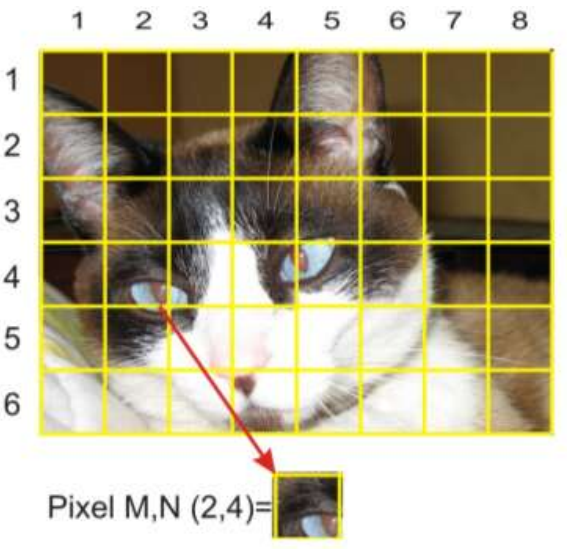
\includegraphics[width=.6\textwidth]{pixel-img}
	\caption{Exemplo de imagem representada como uma matriz (M,N) de pixels, com destaque para o pixel (2,4).}
	\fonte{\cite{img-digital-willians}}
	\label{pixel_img}
\end{figure}


Para que uma imagem analógica (representação real da cena) seja convertida, esta deve sofrer uma separação espacial (amostragem) e em amplitude (quantização) \cite{img-digital-willians}. 

A amostragem é a divisão do plano $(x,y)$ em uma grade (ou matriz bi-dimensional) onde \textit{x} e \textit{y} serão números inteiros. Os pontos da matriz são denominados \textit{pixels} (\textit{PICTure Elements}), como ilustra a \autoref{pixel_img}. Cada pixel representa uma parte da cena real, desta forma a resolução espacial da imagem é proporcional aos valores de M e N correspondentes na matriz (ao exemplo da \autoref{pixel_img}). Em geral a malha de amostragem, o formato dos pixels $(x,y)$, é retangular, mas pode também ser triangular ou mais complexa. Os valores de cada ponto da matriz, coluna \textit{x} e linha \textit{y}, que identificam um único pixel $(M,N)$, devem ser escolhidos de forma a respeitar a relação qualidade da imagem \textit{vs.} espaço de armazenamento, em função da aplicação para a qual a imagem se destina. Para uma imagem digital com 256 níveis de cinza o número de bytes ocupados para armazenar a imagem é o produto da linha, coluna da matriz e 8 bits (unidade mínima de armazenamento digital) \cite{img-digital-willians}. 

Matematicamente, toda imagem em escala de conza é um função $f(x,y)$ da intensidade luminosa, em qualquer parte das coordenadas $(x,y)$, proporcional ao brilho (tons de cinza) da imagem em um determinado ponto \cite{gonzalez_woods}. 

A função  $f(x,y)$  é a multiplicação da iluminância  $i(x,y)$ que é a quantidade de luz que incide sobre o objeto pela refletância  $r(x,y)$  que é fração de luz incidente que o objeto vai refletir ao ponto $(x,y)$. 

Sendo assim, podemos dizer que :

$f(x,y) = i(x,y) * r(x,y)$,
onde $0 < i(x,y)$ e $0 < r(x,y) < 1$ .

Quando se utiliza uma imagem colorida, no padrão RGB por exemplo,  deve se usar uma função $f(x,y)$ para cada banda, R (\textit{Red}), G (\textit{Green}) e B (\textit{Blue}) que são as cores primárias \cite{gonzalez_woods}.

 
\subsection{Formato PNG}\label{subsec:png}

PNG (\textit{Portable Network Graphics} ou "\textit{PNG is Not Giff}") é um formato de representação de imagens do tipo \textit{raster} e foi desenhado para substituir o formato GIF e o TIFF em certa extensão. Uma das vantagens do PNG é o suporte de canal alfa (transparência) de forma eficiente. Além disso, o formato é livre \cite{png}. 

O trabalho da compressão é justamente retirar essas informações redundantes para diminuir o peso do arquivo. Por exemplo, dado um pixel qualquer de uma imagem, possivelmente, a cor ou o valor desse pixel será igual a de vários outros elementos dentro da mesma imagem. Quando a imagem é comprimida, para excluir os pixels de valores iguais, é guardado apenas um valor desse pixel, que é reproduzido para os outros semelhantes, economizando tempo de carregamento \cite{img_compact}. Existem outras técnicas são utilizadas para tal processo.

 \subsection{Vídeo Digital}\label{subsec:videodigi}
 
 Um vídeo é uma sucessão de imagens apresentadas sequêncialmente em um determinado ritmo. O olho humano pode distinguir cerca de 20 imagens por segundo. Deste modo, quando se mostram mais de 20 imagens por segundo, é possível enganar o olho e criar a ilusão de uma imagem em movimento. 
 
 A fluidez de um vídeo se caracteriza pelo número de imagens por segundo (frequência de quadros), expresso em FPS (Frames per second - Quadros por segundo). O vídeo multimídia é geralmente acompanhado de som, ou seja, dados de áudio \cite{ccm_video_digi}.

\subsection{Aquisição da Imagem e de Vídeo}\label{subsec:aquisicao_video}

No processo de aquisição de imagens, tradicionalmente, uma "cena" tridimensional (ou imagem analógica) deve ser capturada por um dispositivo eletrônico, que colhe uma amostragem convertendo-a para uma imagem digital de duas dimensões. Por exemplo, uma câmera digital captando uma cena 3D e convertêndo-a em 2D.

Atualmente o dispositivo de conversão mais usado  é a câmera CCD (\textit{charge coupled device}), que é uma matriz de células semi-condutoras fotossensíveis que trabalham com capacitadores, fazendo um armazenamento da carga elétrica proporcional à energia luminosa incidente \cite{gonzalez_woods}.

A saída deste processo é a imagem do tipo \textit{raster}, pronta pra ser formatada e compactada por alguma representação (PNG, JPG, BPM, etc). 


Na aquisição de vídeos, o mesmo processo descrito acima para imagens é utilizado, com a diferença de que o vídeo é uma fluidez de imagens, sendo assim é necessário aplicar este processo iterativamente. Caso uma única imagem precise ser colhida do vídeo, basta escolher um quadro (descrito na \autoref{subsec:videodigi}) para o processo.

\subsection{Processamento da Imagem}\label{subsec:processamento}

O processamento de imagem é todo o processo que tem uma imagem como entrada e saída, tais como fotografia ou quadros de vídeo \cite{inpe_proc_img}. 

Usa-se para melhorar o aspecto visual de certas feições estruturais para o analista humano ou para performance e para fornecer outros subsídios para a sua interpretação, inclusive gerando produtos que possam ser posteriormente submetidos a outros processamentos \cite{inpe_proc_img}.

O processamento de imagens pode ser dividido em 3 fases básicas: pré-processamento, realce e classificação.
Pré-processamento refere-se ao processamento inicial de dados brutos para calibração radiométrica da imagem, correção de distorções geométricas e remoção de ruído.
Realce visa melhorar a qualidade da imagem, permitindo uma melhor discriminação dos objetos presentes na imagem.
Na classificação são atribuídas classes aos objetos presentes na imagem \cite{inpe_proc_img}.

Nas próximas seções algumas técnicas de processamento de imagens serão abordadas pela sua importância e sua necessidade de uso em algoritmos de detecção e reconhecimento de faces. São elas:

\begin{itemize}
	\item Conversão em Escala de Cinza: considerada uma técnica de pré-processamento, é usada para transformar a imagem para  escala de cinza, o que torna outras operações de processamento mais rápidas e eficientes;
	\item Escalonamento: pré-processamento de correção linear geométrica 2D \cite{lapix_escala};
	\item Equalização: uma técnica de realce de contraste \cite{gonzalez_woods}
	\item Segmentação: recorte da imagem, onde se extraem os objetos relevantes para a aplicação desejada \cite{inpe_proc_img}.
	\item Classificação: uso de classificadores para reconhecer padrões em imagens \cite{drmathew_java_programming}
\end{itemize}

\subsubsection{Conversão em Escala de Cinza}\label{subsubsec:filtros}

Em fotografia, computação e colometria, uma imagem em escala de cinza é uma imagem em que cada valor de pixel é uma única amostra da representação de intensidade de luz \cite{stephen_greyscale}. A seguir são apresentadas três dos vários métodos utilizados para conversão de imagens coloridas para escala de cinza para imagens do tipo \textit{raster}: método escolha de canal, máximo canal e conversão clássica \cite{ricardo_pdi}.

%\vspace*{5cm}
\begin{figure}[h]
	\centering
	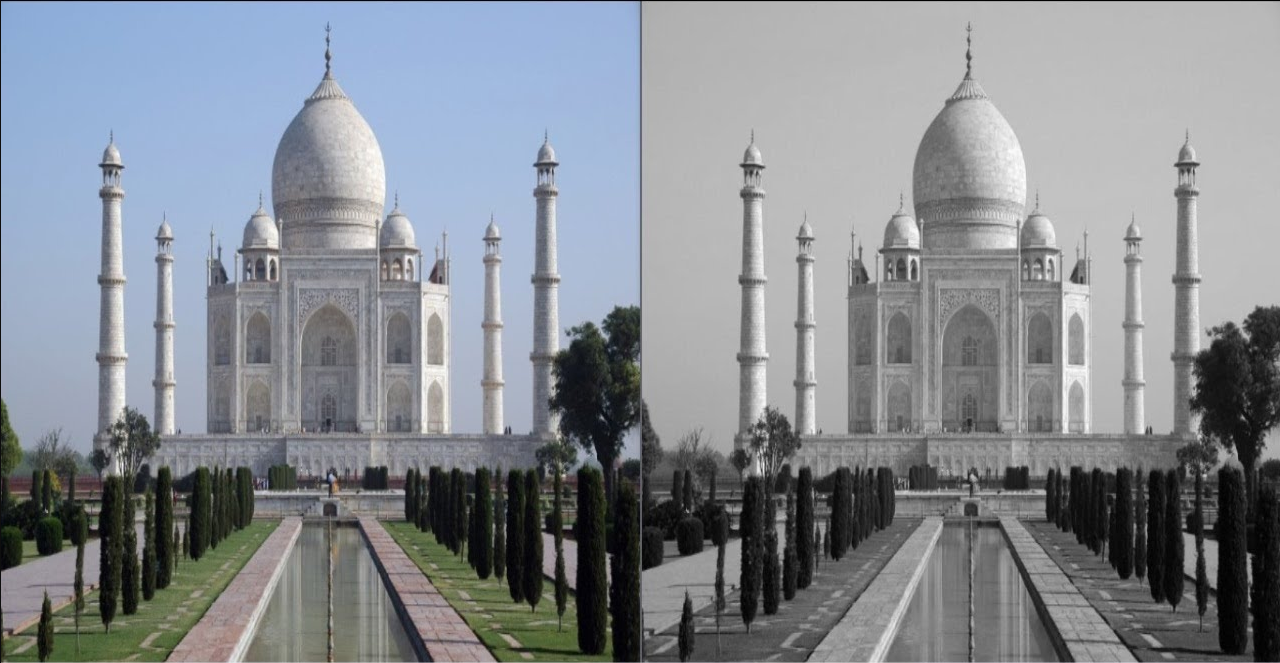
\includegraphics[width=.65\textwidth]{escalacinza}
	\caption{Decomposição dos canais do sistema RBG. }
	\fonte{\cite{ricardo_pdi}}
	\label{escalacinza_img}
\end{figure}

No Método \textbf{Escolha de Canal}, tendo uma imagem do tipo \textit{raster} RGB, umas das formas mais simples para convertê-la em níveis de cinza é escolhendo um dos três canais (\textit{red}, \textit{blue} ou \textit{green}) para ser a imagem resultande, ou seja, a repetiçãao do canal escolhido nos outros dois canais mantendo assim a imagem com três matrizes (em RGB) como mostra a \autoref{escalacinza_img}.	


No Método \textbf{Máximos Canal}, considerando uma imagem RBG, cada pixel "\textit{p}" da matriz da imagem resultante será o de maior valor dentre os pixels da mesma posiçào "\textit{p}" dos três canais do RGB. O resultado da conversão por este metodo é ilustrado na \autoref{maximo_canalimg}.
\begin{figure}[h]
	\centering
	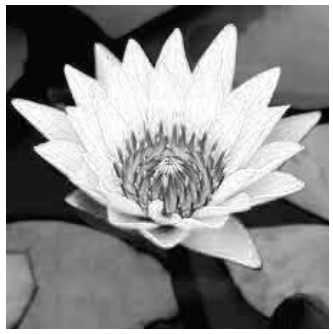
\includegraphics[width=.4\textwidth]{maximo_canal}
	\caption{Conversão em tons de cinza pelo método máximo canal.}
	\fonte{\cite{ricardo_pdi}}
	\label{maximo_canalimg}
\end{figure}	

	
No Método de \textbf{Coversão Clássico} utiliza-se de "pesos" sobre os valores RGB para calcular a resultante "$r$" pela equação $r = 0.29R + 0.59G + 0.11B$. A \autoref{conversao_classica} ilustra o resultado do uso deste método. 
\begin{figure}[h]
	\centering
	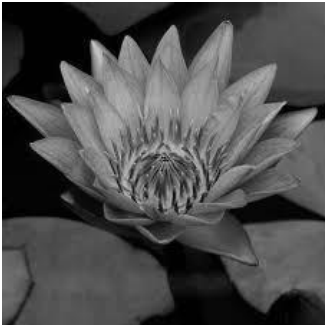
\includegraphics[width=.4\textwidth]{conversao_classica}
	\caption{Conversão em tons de cinza pelo método de conversão clássico}
	\fonte{\cite{ricardo_pdi}}
	\label{conversao_classica}
\end{figure}

Já o Método \textbf{Média de Canal} consiste em calcular a média dos valores RGB de cada pixel e atribuir o resultado ao pixel novamente para cada valor R, G e B, como mostra a \autoref{media_canal}
\begin{figure}[h]
	\centering
	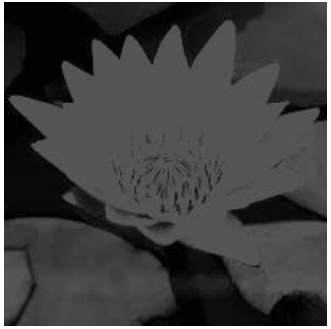
\includegraphics[width=.4\textwidth]{media_canal}
	\caption{Conversão em tons de cinza pelo método de média de canal.}
	\fonte{\cite{ricardo_pdi}}
	\label{media_canal}
\end{figure}

Converter a imagem em escala de cinza torna mais eficientes os subsequente processos, como equalização e aplicação de classificadores \cite{drmathew_java_programming}. 


%-----------------------------------------------


\subsubsection{Escalonamento}\label{subsubsec:escalonamento}

No âmbito de Computação Gráfica e Imagens Digitais e referindo-se a imagens do tipo \textit{raster} (matriciais), o escalonamentro de imagens pode ser interpretado como uma reamostragem ou reconstrução da imagem. A imagem reconstruída pode ser maior ou menor dependendo do fator de escala. Quando uma imagem é diminuida de seu tamanho original, os dados da imagem (pixels) são descartados, e quanto o tamaho da imagem é aumentada, novos dados devem ser inseridos na imagem.
Basicamente esses  novos dados a principio são espaços "vazios" como mosta a \autoref{escalabasico}. 

\begin{figure}[h]
	\centering
	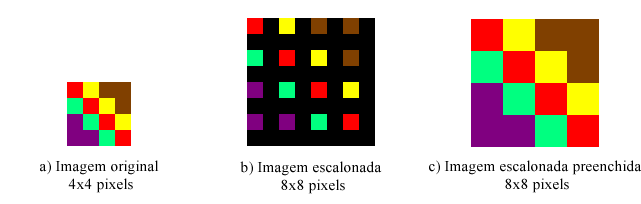
\includegraphics[width=.8\textwidth]{escalabasico}
	\caption{Exemplo de escalonamento de imagem.}
	\fonte{Adaptado de \cite{tech_algo_scaling}}
	\label{escalabasico}
\end{figure}

A principal função de um algoritmo de escalonamento é de prenecher estes espaços "vazios" com pixels de valores coerentes. Para tal utiliza-se técnicas matemáticas de interpolação com os dados da imagem. Interpolação é o processo de estimar valores intermediários de uma função ou sinal discreto amostrado em posições no espaço contínuo \cite{luiz_vizinho}.

Existem várias técnicas de interpolação, dentre elas:

\begin{itemize}
	\item Interpolação do vizinho mais próximo;
	\item Interpolação Bilinear;
	\item Interpolação Bicúbica;
	\item Interpolação Bicúbica Generalizada;	
\end{itemize}

A interpolação do Vizinho Mais Próximo por exemplo, é a maneira mais simples de abordar a problemática da interpolação e consiste em determinar o pixel vizinho mais próximo e assumir um valor de intensidade à este \cite{giassa_escalona}, operado pelo arredondamento da coordenada $x$ pelo inteiro mais próximo $u_0$ e usa a amostra em como estimativa de $g(x)$, como ilustra a \autoref{vizinho_interp}.

\begin{figure}[h]
	\centering
	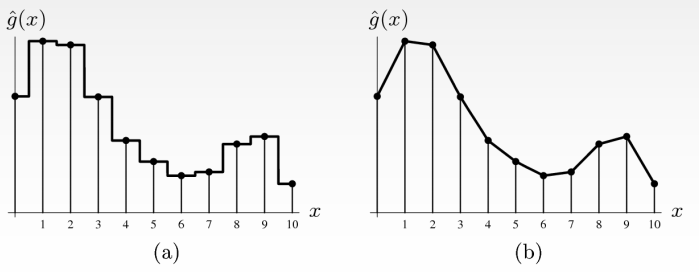
\includegraphics[width=.7\textwidth]{vizinho_interp}
	\caption{(a) Função ou sinal discreto (b) Função ou sinal interpolado }
	\fonte{Adaptado de \cite{giassa_escalona}}
	\label{vizinho_interp}
\end{figure}


\subsubsection{Equalização de Histograma}\label{subsubsec:equalizacao}

O histograma de uma imagem digital é definido segundo \cite{gonzalez_woods} como "uma função discreta $h(r_k)=n_k$ onde  $r_k$ é o k-ésimo valor de intensidade e $n_k$  é o número de pixels da imagem com intensidade $r_k$ e cujos níveis de intensidade desta imagem estejam no intervalo [0, L - 1]". Os Histogramas são a base para várias técnicas de processamento no domínio espacial, onde sua manipulação pode ser utilizada para realce de imagens, além de fornecer dados estatísticos a seu respeito \cite{gonzalez_woods}.

Histograma pode ser visto como uma função de distribuição de frequência ou como uma função de distribuição de probabilidade e é essencialmente um vetor que armazena as ocorrências de cada tom de cinza presentes. Geralmente é mostrado como um gráfico. A equalização de histogramas é "uma operação que melhora o contraste, uniformizando o histograma de forma automática, distribuindo os níveis de cinza existentes e mapeando-os para novos níveis" \cite{gabriel_histograma}.

\begin{figure}[h]
	\centering
	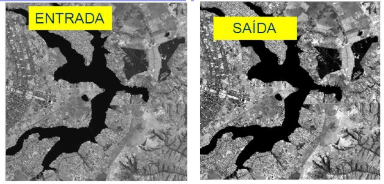
\includegraphics[width=.8\textwidth]{histograma}
	\caption{Exemplo de aplicação de equalização de  histograma.}
%	\fonte{\cite{lapix_escala}}
	\label{fig:histograma}
\end{figure}



\subsubsection{Segmentação}\label{subsubsec:segmentacao}

Em visão computacional, segmentação se refere ao processo recortar uma imagem digital, ou seja, recolher um conjunto de pixels, para simplificar, mudar a representação de uma imagem ou extrair áreas relevantes para facilitar a sua análise. 

Como resultado, cada um dos pixels em uma mesma região é similar com referência a alguma característica ou propriedade computacional, tais como cor, intensidade, textura ou continuidade. Este processo é pré requisito para que reconhecimentos de objetos tenham grandes chances de sucesso \cite{gonzalez_woods}.

\subsubsection{Classificação}\label{subsubsec:classificacao}

Segundo \cite{edinburgh_classifier}, classificação de imagem contextual é um tópico de reconhecimento de padrões em  Visão Computacional. Chama-se "contextual" pois significa que esta abordagem é focada na proximidade com os pixels e sua relação com o "classificador", (contemplado na seção \autoref{subsubsec:elem_haar}). É utilizado efetivamente na detecção de objetos e também pode ser aplicado para a detecção de faces em uma imagem.


%============================================================================================================


\section{Detecção de Faces com Classificadores Haar}\label{sec:deteccao}

Um classificador Haar pode ser treinado para detectar vários tipos de objetos rígidos, definidos, como carros, motos ou partes do corpo humano como olhos ou boca, com altas taxas de sucesso. Não é muito eficiente em reconhecer objetos com ramos tipo arvores, mãos ou objetos camuflados ou contendo pouca textura, contorno e sub-regiões que variam em cor e iluminação \cite{drmathew_java_programming}.

Um classificador bem treinado pode envolver milhares de fotos de alta qualidade com imagens positivas. Para a detecção de faces, isto significa imagens de rostos tiradas de perto que devem ter posições similares com muito pouca variação de fundo (\textit{background} \textit{variation}). Olhos bocas e narizes devem estar na mesma posição em todas as fotos, e estas devem ser do mesmo tamanho. Também é necessário treinar o classificador com um número similar de imagens negativas (isto é, sem rostos).

Existem diversas bibliotecas com classificadores pré-treinados para diferentes objetos, incluindo faces.


\subsection{Os Classificadores Haar (\textit{Haar Features}) }\label{subsubsec:elem_haar}

Os classificadores Haar (ou cacarcterísticas de haar, ou filtro haar) recebem esse nome pela sua similaridade com a \textit{Haar wavelet} (ou ondulação Haar), que consiste em uma sequência de funções quadradas redimensionadas que formam uma familia de ondulações das mais simples possíveis.

 \begin{figure}[h]
 	\centering
 	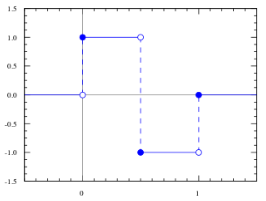
\includegraphics[width=.6\textwidth]{haarwavelet}
 	\caption{Um exemplo de \textit{Haar wavelet}}
	\fonte{Adaptado de \cite{gonzalez_woods}}
 	\label{fig:haarwavelet}
 \end{figure}

Características Haar são basicamente imagens treinadas e usadas para achar objetos similares em outras imagens. Viola e Jones em seu algoritmo \textit{Haar Cascades} (contemplado na seção seguinte), por exemplo, utilizam classificadores retangulares. Cada classificador pode indicar a existência ou a ausência de uma característica em outra imagem. A maior motivação para o uso de características em um objeto ao invés do uso de pixel é que a velocidade da análise de uma imagem baseada no conjunto de sua principais características é muito maior do que a análise baseada sobre seus pixels, devido ao fato do numero de características ser substancialmente inferior em relação ao número de pixels \cite{gustavo_cascata}.

A \autoref{fig:haarfeatures} mostra um classificador Haar em ação.

 \begin{figure}[h]
	\centering
	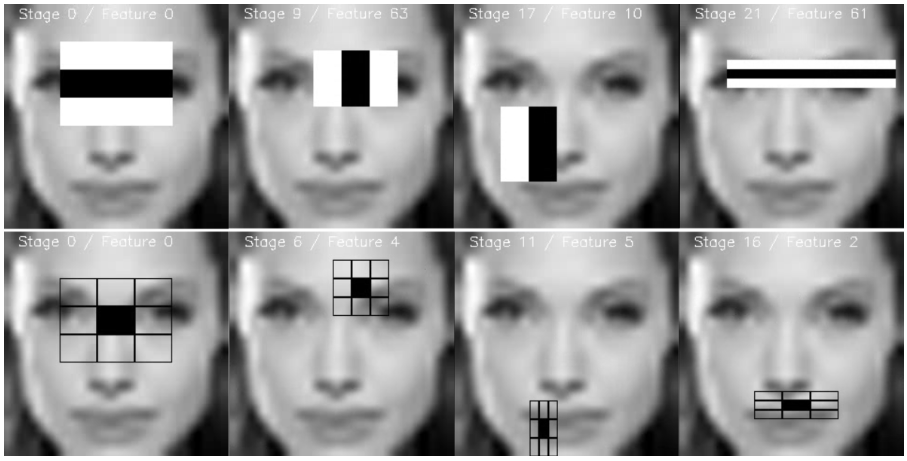
\includegraphics[width=.9\textwidth]{haarfeatures}
	\caption{Classificadores Haar representando características relevantes face}
	\fonte{Biblioteca OpenCV}
	\label{fig:haarfeatures}
\end{figure}

Estes padrões retangulares podem ser escalonados para que caracterísricas de diferentes tamanhos na imagem possam ser detectados usando a mesma abordagem.


\subsection{Algoritmo Viola-Jones (\textit{Haar Cascades Classifier}) }\label{subsubsec:violajones}

O \textit{framework} de detecção de objetos Viola-Jones, apelidado em inglês de \textit{Haar Cascades Classifier}, ou em português Cascata de Classificadores Haar \cite{gustavo_cascata}, foi o primeiro algoritmo de detecção a fornecer detecção de objetos com taxas de sucesso competitivas e em tempo real. Foi proposto em 2001 por Paul Viola e Michael Jones. Apesar de poder detectar uma variedade de classes de objetos, foi desenhada com o objetivo primordial de detectar faces.

Com a utilização das características Haar, o objetivo a ser alcançado é classificar corretamente um dado objeto a partir do conjunto de suas principais características. 

De acordo com \cite{drmathew_java_programming}, o algoritmo funciona com o uso de integrais que são rápidas e eficientes, possibilitando ainda reduzir drasticamente o número de atributos que precisam ser testados para decidir se a imagem contem um objeto (por exemplo uma face). Os testes de atributos da imagem são organizados em "cascatas" também pode ser representado por uma árvore binária, representando o uso das integrais iterativas.

O nó-raiz da árvore binária deve contér um valor representando o teste que se provou ser o melhor em encontrar um objeto durante o treino. Se uma imagem não é rejeitada por este valor teste então a imagem segue para o nó com o segundo melhor valor de teste, e assim sucessivamente. Apenas se a imagem alcançar o fim de todos os nós (ou fim da cascata ou da árvore) sem ser rejeitada, a imagem certamente deverá conter o objeto característico.

O grande ponto negativo é que este algoritmo também detecta os objetos que não são realmente os objetos que se tinha a intenção de detectar \cite{drmathew_java_programming}. Por exemplo, o desenho de um rosto certamente vai ser detectado com uma face, e este desenho não precisa ser muito bem elaborado. As vezes uma disposição de sombras e regiões luminosas aleatórias podem ser detectadas como objetos característicos .

Segundo \cite{gustavo_cascata}, os estágios dentro de uma cascata são criados através da combinação de funções de classificadores Haar previamente treinados. O principal objetivo do uso de cascatas é fazer com que seus estágios iniciais descartem um grande numero de regiões que \textbf{não contém} o objetivo desejado, e estágios mais avançados sejam melhores em evitar um falso positivo na região analisada. 

A \autoref{fig:cascata} representa os $N$ estágios de uma cascata de classificadores. Cada um deles deve descartar ao máximo o número de regiões da imagem que não contém o objeto, a fim de diminuir a quantidade de processamento de outras sub-áreas da imagem original \cite{gustavo_cascata}.

 \begin{figure}[h]
	\centering
	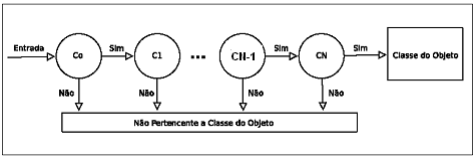
\includegraphics[width=.8\textwidth]{cascata}
	\caption{Cascata de classificadores com estágios (C0, C1, ..., Cn)}.
	\fonte{\cite{gustavo_cascata}}
	\label{fig:cascata}
\end{figure}

O processo para geração da cascata é guiado por um conjunto de metas de detecção e de desempenho. Na prática, uma arquitetura muito simples pode ser usada para produzir uma eficiente cascata de classificadores. O usuário pode informar as taxas mínimas aceitáveis e cada estágio da cascata é treinada junto ao conjunto de características Haar contando com cada vez mais elementos até que se atinjam as taxas de detecção de sucesso e falsos positivos. As taxas são encontradas testando o detector corrente sobre um conjunto de validação. Se a taxa de falsos positivos ainda não for atendida, então um novo estágio subsequente é ativado, coletando todas as falsas detecções encontradas \cite{gustavo_cascata}.

Para que o algoritmo possa detectar o objeto de interesse, é necessário que a imagem seja percorrida diversas vezes em várias direções, assim a cada iteração é analisada uma região de tamanho diferente, chamada \textbf{janela de busca} \cite{gustavo_cascata}. 

O usuário pode definir o tamanho desta janela que deve ser maior ou igual ao tamanho das imagens que foram treinadas na cascata, ou seja, se a cascata foi treinada com imagens positivas de 24x24 pixels, o tamanho mínimo da janela de busca deve seguir a mesma resolução \cite{gustavo_cascata}. As janelas devem funcionar em \textit{threads}, sendo que \textit{n} janelas devem se deslocar no eixo X da imagem e \textit{m} janelas no eixo Y. A quantidade de janelas deve ser o suficiente para ocupar todo o espaço da imagem.

Outro valor que o usuário pode informar é o número de detecções subsequentes necessários para que a região seja considerada a ter o objeto alvo. Reduzir este valor pode aumentar a velocidade de processamento, mas também aumenta as chances de taxas de falsos positivos \cite{drmathew_java_programming}.

O resultado do algoritmo são as posições dos objetos classificados com as características as quais se recebeu treinamento, podendo ser identificados na imagem.


%============================================================================================================


\section{PROCESSO DA ANÁLISE DE COMPONENTES PRINCIPAIS (ACP) OU \textit{EIGENFACES} } \label{sec:recog_faces}

A técnica PCA (Análise de Componentes Principais) foi descrita inicialmente por Karl Pearson em 1901 como solução para alguns problemas biométricos da época, mas ele não propôs nenhuma implementação dessa técnica para um caso com mais de duas variáveis. Em 1933 essa técnica foi descrita por Hotteling, mas os cálculos ainda eram complexos quando se tratava de um problema com dezenas de variáveis. Apenas com o surgimento dos computadores atuais, a técnica ficou mais difundida (\cite{geysilva}). 

O processo de reconhecimento de faces depende de uma fase de treinamento precedente envolvendo imagens faciais com suas identidades associadas. Imagens típicas de treinamento são mostradas na \autoref{fig:trein_img}.
\begin{figure}[h]
	\centering
	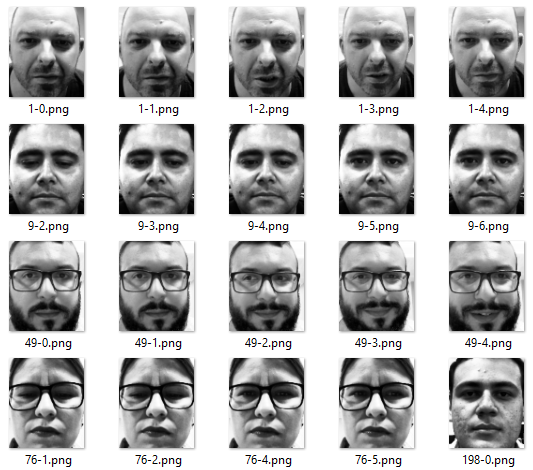
\includegraphics[width=.7\textwidth]{trein_img}
	\caption{Exemplo de imagens típicas de treinamento.}
	\fonte{elaborado pelo autor}
	\label{fig:trein_img}
\end{figure}

É importante que as imagens sejam todas colhidas e orientadas de maneira similar, para que as variações entre as imagens sejam causadas por diferenças entre as faces e não por diferenças  em plano de fundo ou posição facial. Também deve haver uniformidade na posição, clareamento, tamanho e resolução da imagem. É recomendado incluir várias imagens da mesma face mostrando diferentes expressões, como sorrindo ou abrindo a boca. A relação da imagem com o indivíduo pode ser feita de diversas maneiras, uma delas é codificar alguma chave única para o indivíduo junto ao nome da imagem \cite{drmathew_java_programming}. 

O processo de treinamento cria as \textit{EigenFaces}, como mostra a \autoref{someeigen} explicada na  \autoref{subsec:treinrecface}, que são composições das imagens de treinamento que tem a propriedade de acentuar elementos que podem ser distinguidos mais facilmente pelo algoritmo. Uma imagem de face pode gerar várias \textit{EigenFaces}. As imagens de treino da face podem ser representadas por uma sequência de "pesos" (p1, p2, p3, p4, p5, p6), como ilustra a \autoref{fig:eigenpeso}.

\begin{figure}[h]
	\centering
	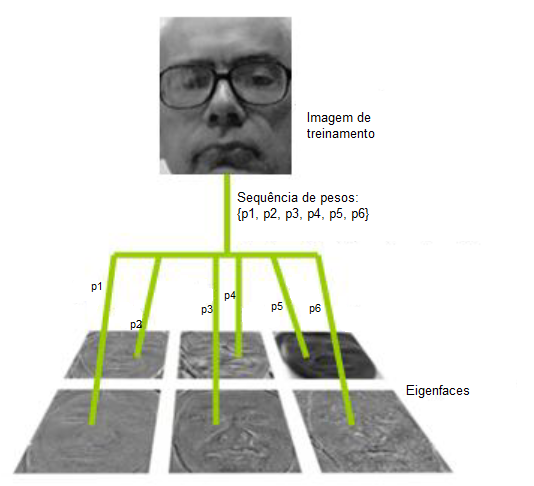
\includegraphics[width=.4\textwidth]{eigenpeso}
	\caption{Exemplo de uma imagem de treinamento representada em uma sequência de pesos de engenfaces.}
	\fonte{Adapdato de \cite{drmathew_java_programming}}
	\label{fig:eigenpeso}
\end{figure}

O objetivo é que a imagem de treinamento pode ser decomposta por uma soma dos pesos das multiplas \textit{EigenFaces}, sendo todos estes pesos salvos como uma sequência.

Nem todas as \textit{EigenFaces} são igualmente importantes - algumas pode contar elementos faciais mais importantes para distinguir faces. Isto quer dizer que não é necessário utilizar todas as eigenfaces para reconhecer uma face, o que permite que uma imagem seja representada por uma pequena quantidade de \textit{EigenFaces}, o que ocupa menos espaço e torna a execução do algoritmo mais rápida. O ponto negativo é que com menos pesos, a probabilidade de se perder importantes elementos faciais também aumenta \cite{drmathew_java_programming}.

Outra maneira de se entender a relação entre \textit{EigenFaces} e as imagens é representa-las em um espaço cartesiado multidimensional (ou um \textit{\textit{EigenSpace}}), como mostra a \autoref{fig:eigenpeso_axis}.

\begin{figure}[h]
	\centering
	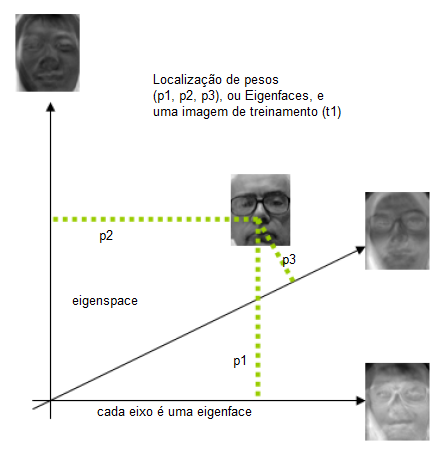
\includegraphics[width=.4\textwidth]{eigenpeso_axis}
	\caption{Exemplo de eigenfaces representadas em um plano cartesiano (\textit{eigenspace}) de 3 dimensões. }
	\fonte{Adapdato de \cite{drmathew_java_programming}}
	\label{fig:eigenpeso_axis}
\end{figure}

Os pesos agora podem ser observados como as coordenadas da imagem de treinamento em um espaço cartesiano multidimensional (\textit{EigenSpace}). Na \autoref{fig:eigenpeso_axis}, existem apenas 3 eixos representando as \textit{EigenFaces} p1, p2 e p3, porém se houvessem 10 \textit{EigenFaces}, haveriam 10 eixos neste espaço.

Após o processo de treinamento das faces vem o processo de reconhecimento. Neste novo processo, uma nova imagem para reconhecimento deve ser decomposta em \textit{EigenFaces}. A sequência de pesos resultante é comparada com cada sequência de pesos que foram previamente disponibilizadas no espaço multidimensional, e o nome associado com o as características mais próximas dos \textit{EigenFaces} treinados é associado \cite{drmathew_java_programming}.

Em outras palavras, em termos de espaço multidimensional, a nova imagem é posicionada no plano cartesiano com suas próprias coordenadas (pesos). Então uma técnica de medida de distância (geralmente a distância Euclidiana, que será abordada na \autoref{subsec:eigenacp}) é utilizada para encontrar o vetor de valores correspondente mais próxima. Sendo assim, uma distância zero seria uma correspondência (reconhecimento) perfeita \cite{drmathew_java_programming}. A \autoref{eigencartesiano} na \autoref{subsec:treinrecface} ilustra este processo.


%=======================================================================================================================

\subsection{O Cálculo da Análise de Componentes Principais (ACP)}\label{subsec:acp}

Segundo \cite{geysilva}, o algoritmo da ACP pode ser dividida em duas fases: a fase de treinamento e a de reconhecimento. Cada fase consiste na realização de processos, descitos as seções abaixo.

\subsubsection{Fase de Treinamento} \label{subsec:treinamento}

Esta fase consiste no procedimento de cinco passos:

%PASSO 1
\textbf{Passo 1 - Preparação dos dados:}  neste passo deve-se preparar os dados das imagens aquisitadas nas condições descritas na seção \autoref{sec:recog_faces} e disponibilizá-las na forma de vetores de \textbf{bytes} para serem manipulados. A \autoref{tabelaxy} exemplifica 2 conjuntos (vetores) de dados que poderiam ser utilizados: o vetor \textit{x} e \textit{y}.

\begin{table}[h]
	\centering
	\caption{Dados dos vetores \textit{x} e \textit{y}.}
	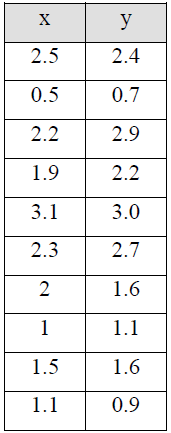
\includegraphics[width=.15\textwidth]{tabelaxy}
	\fonte{\cite{drmathew_java_programming}}
	\label{tabelaxy}
\end{table}

Na \autoref{fig:graphxy} plota-se os valores correspondentes dos vetores \textit{x} e \textit{y} como pontos em um gráfico \cite{drmathew_java_programming}.


\begin{figure}[h]
	\centering
	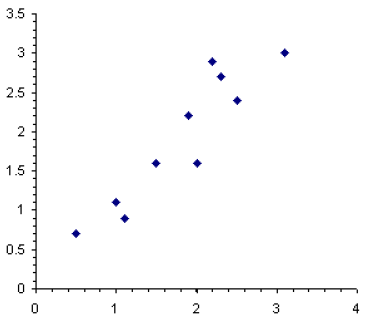
\includegraphics[width=.4\textwidth]{graphxy}
	\caption{Plotagem dos valores de \textit{x} e \textit{y}.}
	\fonte{Adapdato de \cite{drmathew_java_programming}}
	\label{fig:graphxy}
\end{figure}

%PASSO 2
\textbf{Passo 2 - Subtração da Face Média:} neste passo deve-se calcular a face média do conjunto de dados definidos no "Passo 1". A face média ($\Psi$) é definida por:
\begin{center}
	$\Psi = \frac{1}{n} \sum_{1}^{n} X_n$
\end{center}
onde $X_n$ são os conjuntos de dados do "passo 1", sendo $n$ a contagem desses conjuntos. Coma face média calculada  ($\Psi$), deve-se subtraí-la do conjunto de dados ($X_n$):
\begin{center}
	$\Phi_n = X_n - \Psi$
\end{center}
onde $\Phi_n$ é o vetor resultante, tendendo a obter características distintas das imagens. 

%PASSO 3
\textbf{Passo 3 - Cálculo da matriz de covariância:} a covariância é uma medida estatística, generalizada da variância, que compara dois conjuntos de dados. Neste passo deve-se calcular a matriz de covariância para quantificar as diferenças \textbf{entre} os conjutos de dados \cite{drmathew_java_programming}.  Realiza-se o cálculo atravez da formula: 
\begin{center}
	$C = \Phi^T . \Phi$	
\end{center}
onde $\Phi$ é o vetor resultante do "passo 2", $\Phi^T$ é seu equivalente transversal e $C$ é a matriz de covariância resultante \cite{geysilva}.

%Se a fórmula da covariância for aplicada nos dados dos vetores \textit{x} e \textit{y} dados na \autoref{tabelaxy}, o resultado será 0.6154. A parte em que se deve estar atendo é o sinal: se for negativo significa que quando um vetor aumenta em dados, o outro diminui. Quando o valor é positivo, que é o caso, então os dois conjuntos de dados aumentam juntas. Para ilustrar este conceito, 



%Se houverem mais de dois vetores (por exemplo o vetor \textit{x}, \textit{y} e \textit{z}) então a covariância deve ser calculada entra todas os conjuntos de dados, ou seja, calculando cov(x, y), cov(x, z) e cov(y, z). Não há necessidade de calcular cov(y, x), cov(z, x) e cov(z, y) sendo que a definição da equação garante que cov(A, B) é igual a cov(B, A) .

Se a fórmula da covariância for aplicada nos dados dos vetores \textit{x} e \textit{y} dados na \autoref{tabelaxy}, teriam como resultado uma matriz de covariância de dimensões 2x2:
\begin{center}
	$\begin{pmatrix} 0.6166 & 0.6154 \\ 0.6154 & 0.7166 \end{pmatrix}$
\end{center}

%PASSO 4
\textbf{Passo 4 - Cálculo dos auto-vetores e auto-valores:} para que as \textit{eigenfaces} sejam geradas, deve-se decompor a matriz de covariância em outros conjuntos de dados chamados de auto-vetores (ou \textit{eigenvectors}) e auto-valores (ou \textit{eigenvalues}).

Segundo \cite{drmathew_java_programming}, o auto-vetor é um vetor de valores ordinário que quando multiplicado por uma dada matriz, muda de magnitude, enquanto que auto-valor é o valor desta magnitude. Calcula-se os auto-valores atraves de 
 \begin{center}
 	$|\Phi - \lambda I| = 0$	
 \end{center}
onde $\Phi$ é o vetor resultante do "passo 2", $I$ é a matriz identidade da matriz de covariância e $\lambda$ é o auto-valor \cite{geysilva}. Calcula-se os auto-vetores atraves de 
\begin{center}
	$\Phi e = \lambda e$	
\end{center}
onde $\Phi$ é o vetor resultante do "passo 2", $e$ é o auto-vetor e $\lambda$ é o auto-valor \cite{geysilva}.
Neste passo também ordena-se os auto-vetores por ordem de auto-valores (ou seja, por ordem de significância) para facilitar possível futuro descarte \cite{geysilva}.

pode-se observar que o resultado da decomposição da matriz de covariância gereda acima no exempo, como é uma matriz 2x2, possui dois auto-vetores e dois auto-valores:
\begin{center}
	$\begin{pmatrix} -0.7352 \\ 0.6779 \end{pmatrix}$  e 0.049
	
	$\begin{pmatrix} 0.6779 \\ 0.7352 \end{pmatrix}$  e 1.284
\end{center}
Ambos os eigenvetores possuem tamanho unitário.


%PASSO 5!
\textbf{Passo 5 - Projeção dos auto-vetores ao espaço multidimensional:}  neste último passo de treinamento, cada imagem (ou conjunto de dados) de treinamento é projetada no espaço multidimensional de auto-vetores. O Espaço é criado calculando-se através de uma combinação linear de auto-vetores com os vetores originais \cite{geysilva}:
\begin{center}
	$W_n = {e_n}^n (X - \Phi)$	
\end{center}
onde $e$ são os auto-vetores, $X$ é o vetor original de faces de treinamento, $\Phi$ é a face média e $W$ seria o espaço multidimensional resultante.







\begin{comment}
Os dados de \textit{x} e \textit{y} poderiam representar a altura de estudantes, preços de frutas, ou valores numéricos extraídos de uma imagem, por exemplo. O objetivo da demonstração é acentuar as diferenças e similaridades entre os dois vetores de dados em uma abordagem numérica \cite{drmathew_java_programming}. 

Para tal, medidas estatísticas como média e desvio padrão (uma medida que tem o objetivo de espalhar valores acerca da média). Variância é outra medida de espalhamento, que é igual ao desvio padrão ao quadrado:

\begin{figure}[h]
	\centering
	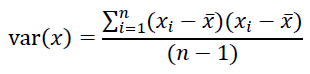
\includegraphics[width=.3\textwidth]{variancia}
%	\caption{Exemplo de eigenfaces representadas em um plano cartesiano (\textit{eigenspace})de 3 dimensões. }
%	\fonte{Adapdato de \cite{drmathew_java_programming}}
	\label{fig:variancia}
\end{figure}

A variável \textit{n} é o número de itens dos vetores (10 de acordo com a \autoref{tabelaxy}), e $\bar{x}$  é a média dos valores d conjunto de dados.

Contudo, a média e a variância fornecem informação apenas sobre a forma dos dados em um único vetor (por exemplo, e média e a variância do vetor \textit{x}), sendo que o objetivo é quantificar as diferenças \textbf{entre} os dois vetores \cite{drmathew_java_programming}.  Justamente a covariância é uma medida estatística, generalizada da variância, que compara dois conjuntos de dados \cite{drmathew_java_programming}:

\begin{figure}[h]
	\centering
	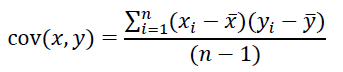
\includegraphics[width=.3\textwidth]{covariancia}
	%	\caption{Exemplo de eigenfaces representadas em um plano cartesiano (\textit{eigenspace})de 3 dimensões. }
	%	\fonte{Adapdato de \cite{drmathew_java_programming}}
	\label{fig:covariancia}
\end{figure}



A maneira padrão de armazenar a covariância entre múltiplos vetores de dados é por uma matriz onde os conjuntos de dados tornam-se os índices das colunas e linhas. Por exemplo, a covariância para os conjuntos de dados x,y e z se tornariam uma matriz de dimensões 3x3 \cite{drmathew_java_programming}:

\begin{figure}[h]
	\centering
	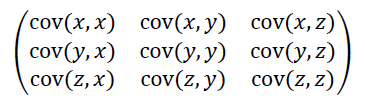
\includegraphics[width=.3\textwidth]{covmatrix}
	%	\caption{Exemplo de eigenfaces representadas em um plano cartesiano (\textit{eigenspace})de 3 dimensões. }
	%	\fonte{Adapdato de \cite{drmathew_java_programming}}
	\label{fig:covmatrix}
\end{figure}

Na diagonal principal, pode-se observar que a covariância é entre o conjunto de dados a própria covariância, que é equivalente à variância nestes dados. Podemos provar isto comparando a variância de x ( var(x) ) e a covariância de x com x ( cov(x) ). A matriz também apresenta simetria em volta da diagonal principal. 


A matriz de covariância é um meio útil de demonstrar a relação entre os conjuntos de dados, mas deve-se obter ainda mais informações para que sejam geradas as \textit{eigenfaces} calculando dois vetores que serão contemplados na seção seguinte: \textit{eigenvectors} e \textit{eigenvalues}.

\subsection{ACP E \textit{Eigenfaces}}\label{subsec:acp-eigen}

Para que as eigenfaces sejam geradas, deve-se transformar a covariância ou outros conjuntos de dados chamados de \textit{eigenvectors} e \textit{eigenvalues}.

Segundo \cite{drmathew_java_programming}, o \textit{eigenvector} é um vetor de valores ordinário que quando multiplicado por uma dada matriz, muda de magnitude, enquanto que \textit{eigenvalue} é apenas um termo para esta magnitude. 

Por exemplo, dada a matriz:

\begin{center}
	$\begin{pmatrix} 2 & 3 \\ 2 & 1 \end{pmatrix}$
\end{center}

O eigenvector para esta matriz é $\begin{pmatrix} 3 \\ 2\end{pmatrix}$, pois quando multiplicado pela matriz acima, o mesmo vetor é retornado o mesmo vetor é retornado se multiplicado por 4:

\begin{center}
	$\begin{pmatrix} 2 & 3 \\ 2 & 1 \end{pmatrix}$ $\times$ $\begin{pmatrix} 3 \\ 2 \end{pmatrix}$ $=$ $4$ $\times$ $\begin{pmatrix} 2 \\ 3\end{pmatrix}$
\end{center}

Sendo assim, 4 é o \textit{eigenvalue} para o \textit{eigenvector}  $\begin{pmatrix} 3 \\ 2\end{pmatrix}$.

Os eigenvectores podem ser encontradas apenas para matrizes quadradas, porém nem todas. Para uma dada matriz n x n, se realmente houver eigenvectores, haverá n. A matriz 2x2 usada de exemplo acima tem dois eigenvetores (e seus valores eigenvalues correspondentes).

A relação eigenvalue pode ser escrita matematicamente como: 

 $\Lambda$ $\nu$  $=$  $\lambda$ $\nu$  

onde $\Lambda$ é a matriz quadrada, $\nu$ é um eigenvetor para A e o valor $\lambda$ é um eigenvalue.

Para usa-los no algoritmo PCA, os eigenvetores devem ser normalizados para que todos eles tenham a mesma unidade de tamanho. Isto é, o eigenvetor acima, $\begin{pmatrix} 3 \\ 2\end{pmatrix}$, tem a unidade de tamanho "falso" de  $\sqrt[]{(3^2 + 2^2)}$ $=$ $\sqrt[]{13}$. Se o vetor for dividido por este valor resultara em um tamanho de unidade \cite{drmathew_java_programming}:

\begin{center}
	$\begin{pmatrix} 3 \\ 2 \end{pmatrix}$ 
	$\div$  
	$\sqrt[]{13}$ $=$ 
	$\begin{pmatrix} 3 / \sqrt[]{13} \\ 2/\sqrt[]{13} \end{pmatrix}$
\end{center}

Se recuperarmos a matriz de covariância que geramos acima:

\begin{center}
	$\begin{pmatrix} 0.6166 & 0.6154 \\ 0.6154 & 0.7166 \end{pmatrix}$
\end{center}

pode-se observar que, com é uma matriz 2x2, possui dois eigenvetores e eigenvalues:

\begin{center}
$\begin{pmatrix} -0.7352 \\ 0.6779 \end{pmatrix}$  e 0.049

$\begin{pmatrix} 0.6779 \\ 0.7352 \end{pmatrix}$  e 1.284
\end{center}

Ambos os eigenvetores possuem unidade de tamanho.


\subsubsection{Utilizando Eigenfaces como Componente Principal}\label{subsec:eigenacp}
\end{comment}


Observando novamente a plotagem dos vetores x e y contemplados na \autoref{fig:graphxy}, se a média destes conjuntos de dados ($\bar{x}$ e $\bar{y}$) for subtraído de seus valores, estes dados então seriam \textbf{normalizados}. Isto também quer dizer que as linhas que representam os vetores \textit{x} e \textit{y} são transladados para o centro como mostra a \autoref{fig:graphxy2}. 

\begin{figure}[h]
	\centering
	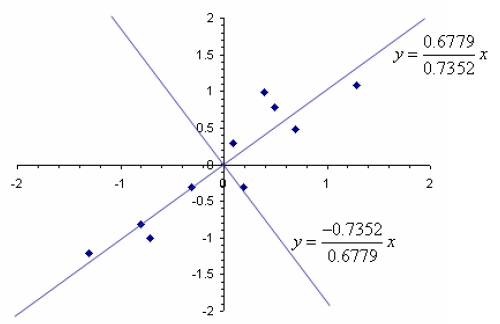
\includegraphics[width=.5\textwidth]{graphxy2}
	\caption{Plotagem normalizada dos dados de \textit{x} e \textit{y} com eigenvetores.}
	\fonte{\cite{drmathew_java_programming}}
	\label{fig:graphxy2}
\end{figure}

Os dois auto-vetores pode ser adicionados ao gráfico como linhas convertendo os vetores em equações. 
$\begin{pmatrix} -0.7352 \\ 0.6779 \end{pmatrix}$ torna-se $y$ $=$ $\frac{-0.7352}{0.6779}$$x$  e $\begin{pmatrix} 0.6779 \\ 0.7352 \end{pmatrix}$ torna-se $y$ $=$ $\frac{0.6779}{0.7352}$$x$.

Os dados normalizados e as duas equações são ilustradas na \autoref{fig:graphxy2} como linhas azuis. 

Observa-se que na \autoref{fig:graphxy2} demonstra como os auto-vetores acentuam as relações entre os conjuntos de dadose indicam como estes se espalham nas coordenadas do espaço multidimensional. Este espalhamento facilita a distinção dos dados \cite{drmathew_java_programming}.

Dos dois auto-vetores marcados em azul, a linha $\frac{0.6779}{0.7352}$$x$ é a mais útil, pois os dados estão mais espalhados acerca do trajeto desta linha. Isto pode ser confirmado numericamente observando o auto-valor associado com seu auto-vetor: o auto-valor (1.284) é um melhor indicador de espalhamento pois é o maior dentre os dois auto-valores.

A outra linha, $\frac{-0.7352}{0.6779}$$x$, contribui com a informação demonstrando como os dados são espaçados para direita ou esquerda do auto-vetor principal (a linha $\frac{0.6779}{0.7352}$$x$). Entretanto, trata-se de um componente menos importante no espalhamento de dados, assim como indica seu auto-valor (0.049) \cite{drmathew_java_programming}.

O auto-vetor com o maior auto-valor (no caso a linha $\frac{0.6779}{0.7352}$$x$, ou o vetor $\begin{pmatrix} 0.6779 \\ 0.7352 \end{pmatrix}$) é chamado de \textbf{componente principal} do conjunto de dados. Isto é, os auto-vetores e auto-valores são efetivamente utilizados para performar uma análise de componente principal nos conjuntos de dados \cite{drmathew_java_programming}.

Todos os auto-vetores extraídos da matriz são perpendiculares. Isto significa que é possível rotacionar (talvez refletir) os dados para que os eigenvetores tornem-se alinhados com os eixos. Se este componente principal $\begin{pmatrix} 0.6779 \\ 0.7352 \end{pmatrix}$ for rotacionado e refletido para que seja alinhado com o eixo y, resulta-se em uma plotagem mostrada na \autoref{fig:graphxy3}:

\begin{figure}[h]
	\centering
	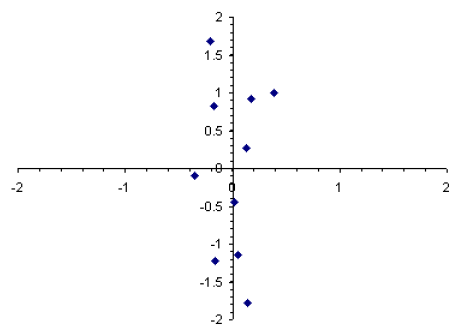
\includegraphics[width=.5\textwidth]{graphxy3}
	\caption{Versão rotacionada e refletida da \autoref{fig:graphxy2}}
	\fonte{\cite{drmathew_java_programming}}
	\label{fig:graphxy3}
\end{figure}

Observando a \autoref{fig:graphxy3}, o ponto mais próximo da origem se situa na coordenada (0.13, 0.27). Pode-se afirmar que também que este ponto tem uma sequência de pesos relativos a cada auto-vetor, no caso, a sequência {0.13, 0.27}.

Tanto a denotação de coordenadas quanto a de pesos pode ser usada para representar as \textit{eigenfaces} - como contemplado anteriormente, na \autoref{fig:eigenpeso} foi dado o exemplo em que uma imagem é uma sequência de pesos de seis \textit{eigenfaces}, enquanto que, alternativamente, na  \autoref{fig:eigenpeso_axis} é representada em coordenadas de um espaço de 3 dimensões, sendo que cada eixo é definido por uma \textit{eigenface} (ou \textit{auto-vetor}) \cite{drmathew_java_programming}.



\subsubsection{O Reconhecimento}\label{subsec:reconhecimento}

O processo de reconhecimento pode ser dividido em 3 passos:

\textbf{Passo 1 - Preparação dos dados:} converter a imagem da nova face em um vetor de consulta $Q$.


\textbf{Passo 2 - Projeção do novo vetor no espaço:} neste passo realiza-se a combinação linear de auto-vetores com o novo vetor de consulta $Q$ por:
\begin{center}
	$W_n = {e^T_n} (Q - \Phi)$
\end{center}
sendo $e$ os auto-vetores, $Q$ o vetor de consulta, e $\Phi$ a face média.

\textbf{O terceiro passo} é comparar a distância entre o descitor do vetor de consulta com cada um dos descitores armazenados na vase de dados. 

%O processo de reconhecimento consiste em recolher novos conjutos de dados (no caso, uma nova face), e utilizando os dados processados até agora e representados na \autoref{fig:graphxy3}, deve-se comparar os dois novos conjuntos de dados (a nova face e os eigenfaces ou eigenvetores) fazendo uso de medidas de distância. 

Existem algumas técnicas de medidas de distância, dentre elas, há uma simples chamada \textbf{Distância Euclidiana}. Esta medida nada mais é do que a distância mínima entre dois pontos no espaço (uma linha reta). A distância euclidiana entre os pontos $P = (p_1, p_2, ..., p_n)$ $Q = (q_1, q_2, ..., q_n)$ é definida como:

\begin{center}
	$\sqrt[]{(p_1 - q_1)^2 + (p_1 - q_1)^2 + ... + (p_n - q_n)^2}$ $=$ $\sqrt[]{ \sum_{i=1}^{n} (p_i - q_i)^2 }$ 
\end{center}

O resultado desta medida é utilizada para calcular a taxa de sucesso de uma comparação, sendo assim uma distância nula representaria uma equivalência perfeita.

%Contudo, em aplicações na vida real, deve-se reduzir o tamanho dos dados, pois existem informações irrelevantes e a tarefa de reconhecimento pode ser executada mais rapidamente enquanto retém informações suficientes para distinguir entre os pontos quando comparados com os novos conjuntos de dados.

\begin{comment}
A técnica consiste em reter todas as coordenadas dos dados, mas reduzir a dimensionalidade do eigenspace, isto é, subtrair o número de eixos do plano cartesiano. Este processo é equivalente a subtrair algumas eingenfaces, mas como citado anteriormente, os enigenvalues de menor intensidade não tem influência no espalhamentos dos dados no plano, sendo pouco significativos para o reconhecimento, e portanto podem ser removidos.

Portanto, os dados mostrados na  \autoref{fig:graphxy3} possuem os seguintes eigenvetores e eigenvalores:

\begin{center}
$\begin{pmatrix} -0.7352 \\ 0.6779 \end{pmatrix}$  e 0.049

$\begin{pmatrix} 0.6779 \\ 0.7352 \end{pmatrix}$  e 1.284
\end{center}

Observando que o primeiro \textit{eigenvector} foi rotacionado em direção ao eixo $x$, e o segundo \textit{eigenvector} em direção ao eixo $y$, se o primeiro \textit{eigenvector} que contribui muito pouco para a informação de espalhamento (devido ao seu pequeno \textit{eigenvalue}) for descartado junto ao seu eixo, os dados deste \textit{eigenvcetors} são projetados para o eixo $y$, resultando na plotagem da \autoref{fig:graphxy4}

\begin{figure}[h]
\centering
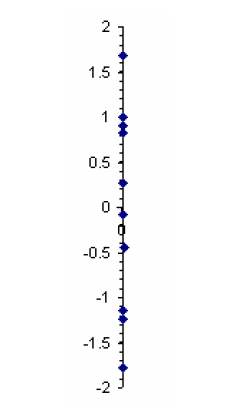
\includegraphics[width=.2\textwidth]{graphxy4}
\caption{Dados da \autoref{fig:graphxy3} projetados em direção ao eixo y.}
\fonte{\cite{drmathew_java_programming}}
\label{fig:graphxy4}
\end{figure}


Apesar dos eixos serem eliminados, seus dados ainda estão presentes e espalhados o suficiente para que o novo conjunto de dados seja comparado com o uso da distância euclidiana.

Considerando que um novo conjunto de dados adicionado com os valores do vetor \textit{z} = (2.511, 2.411), e estes conjuntos passarem pelos mesmos processos que os vetores \textit{x} e \textit{y}, e por fim normalizado e projetado assim como mostra a \autoref{fig:graphxy2} e \autoref{fig:graphxy3}, plotando-o no mesmo espaço resulta na \autoref{fig:graphxy5}.

\begin{figure}[h]
\centering
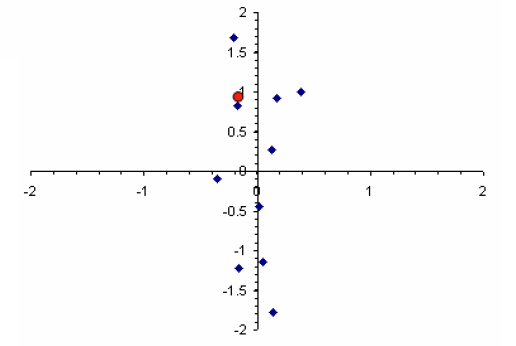
\includegraphics[width=.5\textwidth]{graphxy5}
\caption{Plotagem dos novos dados com os dados de treino transformados.}
\fonte{\cite{drmathew_java_programming}}
\label{fig:graphxy5}
\end{figure}

A \autoref{fig:graphxy5} é a mesma que a \autoref{fig:graphxy3} com a adição de um novo ponto vermelho que indica a ccoordenada do novo conjunto de dados do vetor \textit{z}, posicionada logo acima do ponto (-0.1751, 0.8280), que por sua vez começou como um ponto de treinamento de pesos (2.5, 2.4), informada nos conjuntos de dados \textit{x} e \textit{y}. Isto quer dizer que o novo conjunto de dados \textit{z} (2.511, 2.411) possui a menor distância euclidiana com o conjunto de treinamento (2.5, 2.4). 

A real vantagem dos eigenvetores é quando a dimensionalidade do espaço (eigenspace) torna-se extremamente grande. No presente exemplo foi utilizado uma dimensionalidade dois, enquanto que em aplicações reais com imagem os eixos podem aumentar para valores como 40 mil \cite{drmathew_java_programming}.

Com tamanha dimensão e portanto, quantidade de eixos, como citado anteriormente, pode-se eliminar alguns eixos dependendo de seus valores eingenvalues (se forem pequenos, podem ser considerados dispensáveis). Se por uma hipótese isto for feito neste exemplo incluindo o novo conjunto dados \textit{z}, a plotagem do resultado seria como na \autoref{fig:graphxy6} abaixo:

\begin{figure}[h]
\centering
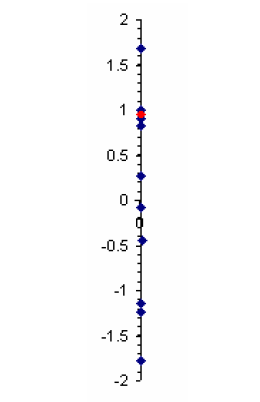
\includegraphics[width=.2\textwidth]{graphxy6}
\caption{Plotagem dos conjuntos de dados \textit{x}, \textit{y} e \textit{z}, trasnformados e projetados no eixo do Componente Principal}
\fonte{\cite{drmathew_java_programming}}
\label{fig:graphxy6}
\end{figure}

A \autoref{fig:graphxy6} é similar à \autoref{fig:graphxy4} com exceção do ponto vermelho (novo dado). Pode-se observar nesta figura o problema potencial em se reduzir a dimensionalidade: a probabilidade de erros aumenta tornando difícil de decidir qual ponto de treinamento é que possui a menor distância euclidiana. Outro fator da equação da distância euclidiana é que se utiliza de um parâmetro para definir quando dois pontos estão perto. Se um valor alto é definido então diversos pontos podem estar dentro do alcance aceitável do novo dado \cite{drmathew_java_programming}.


\subsection{EigenVectors para EigenFaces}\label{subsec:vectoface}

O transformação dos valores numéricos gerados na ACP para imagens EigenFaces nao são necessário para os algoritmos apresentados. Essa transformação serve apenas para satisfazer olhos humanos, ou seja, uma tentativa de observar em imagens os valores gerados pela teoria.


Essencialmente, deve-se converter a imagem para um conjunto de dados, como os vetores $ x $ e $ y $ apresentados na \autoref{tabelaxy}, e performar o algoritmo ACP como descrito anteriormente. A translação de uma imagem para um conjunto de dados é feita tratando esta como um vetor de duas dimensões, e em seguida mapear para um vetor unidimensional como sugere a \autoref{fig:2dto1d}:

\begin{figure}[h]
\centering
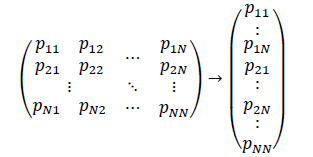
\includegraphics[width=.38\textwidth]{2dto1d}
\caption{Conversão de imagem para conjunto de dados. A variável $P$ seria a representação de um pixel.}
\fonte{\cite{drmathew_java_programming}}
\label{fig:2dto1d}
\end{figure}

Supondo que a imagem tem o tamanho de 200x200 pixels em escala de cinza, o conjunto de dados resultante residirá em um \textit{eigenspace} de 40 mil dimensões, o que acarretará na geração de 40 mil \textit{eigenvectors}, cuja a maioria possui um \textit{eigenvalue} desconsiderável ou insignificante, podendo assim ser descartados. Isto facilitará o processamento da imagem e a utilização da técnica. 

Em geral, supondo que uma imagem quadrada em escala de cinza tem o tamanho de  $ N $ pixels, então $N^2$ eigenvetors serão criados. No seguinte exemplo, será assumido que existem $ M $ imagens:

A técnica consiste em "dividir" a matriz de covariância que é ($ N^2 x N^2 $) em duas matrizes de ($ N^2 x M $) e ($ M x N^2 $). 


\end{comment}




%============================================================================================================

\section{Considerações Finais}\label{sec:revbib_consid_finais}

Neste capítulo foram apresentados os conceitos necessários para o entendimento de todo o processo de Reconhecimento de Faces, constituído de outros sub processos como aquisição de imagem e vídeo, processamento e  classificação de imagens, detecção da face, treinamento e por fim o reconhecimento efetivo da face.

Os algoritmos de detecção de face Viola-Jones, e o de reconhecimento de faces EigenFaces que utiliza o método matemático ACP (Análise de Componentes Principais), foram detalhados na ordem sequêncial de seus processos utilizando exemplos.

No próximo capítulo abordará o plano de materiais e métodos elaborado a partir do conhecimento adquirido no \autoref{ch:rev-bibs}.























